\documentclass[tikz,border=3.14mm,margin=0pt,fontsize=12pt]{standalone}
\usepackage[utf8]{inputenc}
\usepackage{physics}
\usepackage{amsmath}
\usepackage{tikz}
\usepackage{mathdots}
\usepackage{yhmath}
\usepackage{cancel}
\usepackage{color}
\usepackage{siunitx}
\usepackage{array}
\usepackage{multirow}
\usepackage{amssymb}
\usepackage{gensymb}
\usepackage{tabularx}
\usepackage{extarrows}
\usepackage{booktabs}
\usepackage{fontspec}

\usetikzlibrary{fadings}
\usetikzlibrary{patterns}
\usetikzlibrary{shadows.blur}
\usetikzlibrary{shapes}
\usetikzlibrary{arrows.meta}
\usetikzlibrary{positioning}
\usetikzlibrary{calc,decorations.pathreplacing,shapes.misc}

\newcommand{\xmark}{\ding{55}}%
\newcommand{\rulesep}{\unskip\ \vrule\ }

\setlength{\textfloatsep}{6.0pt plus 1.0pt minus 1.0pt}
\setlength{\intextsep}{3.0pt plus 0.5pt minus 0.5pt}

\newfloat{Algorithm}{t!}{lop}

\lstdefinelanguage{All}[]{C}{
  morekeywords={if,then,else,match,with,let,in,fn,type,i32,i8,List,lnode,Str,clnode,u32}
}

\lstnewenvironment{allLangEnvFoot}{\lstset{language=All,basicstyle=\footnotesize\ttfamily,mathescape=true}}{}
\lstnewenvironment{allLangEnvScript}{\lstset{language=All,basicstyle=\scriptsize\ttfamily,mathescape=true}}{}

\lstnewenvironment{myexample}{\lstset{basicstyle=\ttfamily}}{}
\lstnewenvironment{myexamplesmall}{\lstset{basicstyle=\footnotesize\ttfamily}}{}
\lstnewenvironment{myexamplescriptsz}{\lstset{basicstyle=\scriptsize\ttfamily}}{}

\lstset{%
    language     = C,
    keywordstyle = \color{myastral},
    stringstyle  = \color{red},
    breaklines = false,
    commentstyle=\color{mygreen},
    keepspaces=true,
    escapeinside = ~~,
    showlines = true,
%    numbers=left,
%    numberstyle=\tiny\color{mygray},
%    numbersep=2pt,
}

\usepackage{stackengine}
\usepackage{backnaur}
\usepackage{xcolor}

%https://tex.stackexchange.com/questions/123219/writing-above-and-below-a-symbol-simultaneously
\newcommand\stackrqarrow[2]{%
    \mathrel{\stackunder[2pt]{\stackon[1pt]{$\rightsquigarrow$}{$\scriptscriptstyle#1$}}{%
            $\scriptscriptstyle#2$}}}
\usetikzlibrary{arrows, quotes,shapes,positioning, calc}

\newcommand{\toolName}{S2C}%
\newcommand{\sumDtor}{\underline{\tt if}-\underline{\tt then}-\underline{\tt else}}%
\newcommand\sumDtorExpr[3]{\underline{\tt if} #1 \underline{\tt then} #2 \underline{\tt else} #3}%
\newcommand{\recursiveRelations}{recursive relations}%
\newcommand{\recursiveRelation}{recursive relation}%
\newcommand{\SpecL}{Spec}%
\newcommand{\indEq}{\sim}%
\newcommand\indEqDepth[1]{\sim_#1}%
\newcommand\indEqUapprox[1]{\approx_#1}%
\newcommand\depthBound[2]{\Gamma_#1(#2)}%
\newcommand\Reachable[2]{$Reachable_{#1}$(#2)}%
\newcommand\ReachableMath[2]{Reachable_{#1}(#2)}%
\newcommand\structPointer[4]{{\tt #1} \overset{#2}{\rightarrow}_{#3} {\tt #4}}
\newcommand{\seriesEqual}{=}%
\newcommand{\pointsTo}{\rightsquigarrow}
\newcommand{\interfere}{\diamond}
\newcommand\HoareTriple[3]{\{#1\}(#2)\{#3\}}
\newcommand\Lift[4]{{\tt #1}_{#2}^{\tt #3}{(#4)}}

\newcommand*\circled[1]{\tikz[baseline=(char.base)]{
            \node[shape=circle,draw,inner sep=1pt] (char) {#1};}}
\newcommand*\inv[1]{\tikz[baseline=(char.base)]{
\node[shape=rounded rectangle,draw,inner sep=2pt] (char) {\scriptsize {\tt #1}};}}
\newcommand*\pred[1]{\fbox{\scriptsize {\tt #1}}}

\newcommand\Tstrut{\rule{0pt}{2.7ex}}         % = `top' strut
\newcommand\Bstrut{\rule[-1.2ex]{0pt}{0pt}}   % = `bottom' strut

\definecolor{myastral}{RGB}{46,116,181}
\definecolor{myolive}{named}{olive}
\definecolor{mygreen}{rgb}{0,0.6,0.2}
\definecolor{mygray}{rgb}{0.5,0.5,0.5}
\definecolor{myred}{rgb}{0.8,0,0.2}

\newtheorem{theorem}{Theorem}

\newcommand\NonTerm[1]{$\langle$#1$\rangle$}%
\newcommand\Term[1]{{\tt #1}}%

\tikzset{
    ttinner/.style args={#1:#2}{draw,circle,inner sep=0.2mm,label={#1,inner sep=0.1mm:\scriptsize #2}},
    ttleaf/.style={font=\footnotesize},
    ttannot/.style={near start,align=center,font=\scriptsize},
    position/.style args={#1:#2 from #3}{
        at=(#3.#1), anchor=#1+180, shift=(#1:#2)
    },
    show control points/.style={
        decoration={show path construction, curveto code={
                \draw [blue, dashed]
                    (\tikzinputsegmentfirst) -- (\tikzinputsegmentsupporta)
                    node [at end, cross out, draw, solid, red, inner sep=2pt]{};
                \draw [blue, dashed]
                    (\tikzinputsegmentsupportb) -- (\tikzinputsegmentlast)
                    node [at start, cross out, draw, solid, red, inner sep=2pt]{};
            }
        },
        postaction=decorate
    },
}

\begin{document}

\tikzset{every picture/.style={line width=0.40pt}} %set default line width to 0.75pt     

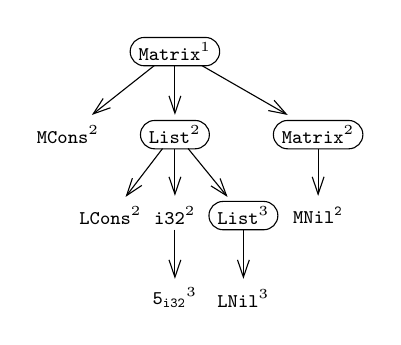
\begin{tikzpicture}[x=0.75pt,y=0.75pt,yscale=-1,xscale=1]
%uncomment if require: \path (0,581); %set diagram left start at 0, and has height of 581


% Text Node
% \draw     (89,341) .. controls (89,339.34) and (90.34,338) .. (92,338) -- (122,338) .. controls (123.66,338) and (125,339.34) .. (125,341) -- (125,350) .. controls (125,351.66) and (123.66,353) .. (122,353) -- (92,353) .. controls (90.34,353) and (89,351.66) .. (89,350) -- cycle  ;
\draw (107,345.5) node  [font=\scriptsize]  {\inv{${\tt Matrix}^1$}};
% Text Node
\draw (55.5,385.5) node  [font=\scriptsize]  {${\tt MCons}^2$};
% Text Node
% \draw     (158,381) .. controls (158,379.34) and (159.34,378) .. (161,378) -- (191,378) .. controls (192.66,378) and (194,379.34) .. (194,381) -- (194,390) .. controls (194,391.66) and (192.66,393) .. (191,393) -- (161,393) .. controls (159.34,393) and (158,391.66) .. (158,390) -- cycle  ;
\draw (176,385.5) node  [font=\scriptsize]  {\inv{${\tt Matrix}^2$}};
% Text Node
\draw (176,424.5) node  [font=\scriptsize]  {${\tt MNil^2}$};
% Text Node
% \draw     (95,381) .. controls (95,379.34) and (96.34,378) .. (98,378) -- (116,378) .. controls (117.66,378) and (119,379.34) .. (119,381) -- (119,390) .. controls (119,391.66) and (117.66,393) .. (116,393) -- (98,393) .. controls (96.34,393) and (95,391.66) .. (95,390) -- cycle  ;
\draw (107,385.5) node  [font=\scriptsize]  {\inv{${\tt List}^2$}};
% Text Node
\draw (76,424.5) node  [font=\scriptsize]  {${\tt LCons}^2$};
% Text Node
\draw (107,424.5) node  [font=\scriptsize]  {${\tt i32}^2$};
% Text Node
% \draw     (128,420) .. controls (128,418.34) and (129.34,417) .. (131,417) -- (149,417) .. controls (150.66,417) and (152,418.34) .. (152,420) -- (152,429) .. controls (152,430.66) and (150.66,432) .. (149,432) -- (131,432) .. controls (129.34,432) and (128,430.66) .. (128,429) -- cycle  ;
\draw (140,424.5) node  [font=\scriptsize]  {\inv{${\tt List}^3$}};
% Text Node
\draw (107,464) node  [font=\scriptsize]  {${\tt 5_{i32}}^3$};
% Text Node
\draw (140,464.5) node  [font=\scriptsize]  {${\tt LNil}^3$};
% Connection
\draw  [-{Straight Barb[length=2.2mm, width=1.5mm]}]  (119.94,352.2) -- (161.33,376) ;
% Connection
\draw  [-{Straight Barb[length=2.2mm, width=1.5mm]}]   (97.1,352.2) -- (67,376) ;
% Connection
\draw  [-{Straight Barb[length=2.2mm, width=1.5mm]}]  (176,392.2) -- (176,415) ;
% Connection
\draw  [-{Straight Barb[length=2.2mm, width=1.5mm]}]  (107,392.2) -- (107,415) ;
% Connection
\draw  [-{Straight Barb[length=2.2mm, width=1.5mm]}]  (113.35,392.2) -- (132.36,415.5) ;
% Connection
\draw  [-{Straight Barb[length=2.2mm, width=1.5mm]}]   (101.04,392.2) -- (83.21,415.5) ;
% Connection
\draw  [-{Straight Barb[length=2.2mm, width=1.5mm]}]  (107,431.2) -- (107,455) ;
% Connection
\draw  [-{Straight Barb[length=2.2mm, width=1.5mm]}]  (140,431.2) -- (140,455) ;
% Connection
\draw  [-{Straight Barb[length=2.2mm, width=1.5mm]}]  (107,352.2) -- (107,376) ;

\end{tikzpicture}


\end{document}
